\documentclass[10pt,a4paper]{article}

\usepackage[margin=22mm]{geometry}
\usepackage{amsmath,amssymb}
\usepackage{graphicx}
\usepackage{booktabs}
\usepackage{longtable}
\usepackage{caption}
\usepackage{xcolor}
\usepackage{titlesec}
\usepackage{enumitem}
\usepackage{fancyhdr}
\usepackage{siunitx}
\usepackage[hidelinks]{hyperref}

\newcommand{\INR}[1]{Rs.\,#1}

\definecolor{accent}{HTML}{16407A}

\titleformat{\section}{\normalfont\Large\bfseries\color{accent}}{\thesection}{0.6em}{}
\titleformat{\subsection}{\normalfont\large\bfseries}{\thesubsection}{0.6em}{}

\pagestyle{fancy}
\fancyhf{}
\lhead{\small\color{accent}isonavi-rov \textbar{} Technical Design Report}
\rhead{\small\thepage}
\renewcommand{\headrulewidth}{0.4pt}

\renewcommand{\topfraction}{0.92}
\renewcommand{\bottomfraction}{0.85}
\renewcommand{\textfraction}{0.06}
\renewcommand{\floatpagefraction}{0.80}
\setcounter{topnumber}{3}
\setcounter{bottomnumber}{2}
\setcounter{totalnumber}{5}

\captionsetup{font=small,labelfont={bf,color=accent}}
\sisetup{detect-all}
\setlist{nosep,leftmargin=1.4em}

% Generated by simulation/eval/make_rov_metrics.py. Do not edit.
\newcommand{\mballast}{1.36}
\newcommand{\mbeam}{44}
\newcommand{\mbg}{45}
\newcommand{\mbomlines}{34}
\newcommand{\mcadbuoybuilt}{2.272}
\newcommand{\mcadclash}{0}
\newcommand{\mcadenvb}{44.0}
\newcommand{\mcadenvh}{33.0}
\newcommand{\mcadenvl}{66.0}
\newcommand{\mcadhull}{53.4}
\newcommand{\mcadhullbuilt}{3.449}
\newcommand{\mcadoutflow}{4}
\newcommand{\mcadparts}{37}
\newcommand{\mcadplate}{10.0}
\newcommand{\mcapthrust}{24.3}
\newcommand{\mcapw}{800}
\newcommand{\mcostbuild}{1,14,229}
\newcommand{\mcostcont}{12,463}
\newcommand{\mcostelectronics}{32,150}
\newcommand{\mcostframe}{7,650}
\newcommand{\mcosthull}{8,600}
\newcommand{\mcostinhouse}{21,450}
\newcommand{\mcostpropulsion}{25,472}
\newcommand{\mcostsurface}{31,432}
\newcommand{\mcosttest}{10,400}
\newcommand{\mcosttether}{8,925}
\newcommand{\mcosttotal}{1,37,092}
\newcommand{\mcostvehicle}{73,872}
\newcommand{\mdisplaced}{10.70}
\newcommand{\mfoam}{2.15}
\newcommand{\mframedrag}{21.9}
\newcommand{\mfuse}{25}
\newcommand{\mgateclearone}{54}
\newcommand{\mgateclearoneavail}{100}
\newcommand{\mgateclearonehalf}{30}
\newcommand{\mgateclearonehalfavail}{100}
\newcommand{\mgatecleartwo}{46}
\newcommand{\mgatecleartwoavail}{96}
\newcommand{\mgatemidone}{24}
\newcommand{\mgatemidoneavail}{100}
\newcommand{\mgatemidonehalf}{30}
\newcommand{\mgatemidonehalfavail}{100}
\newcommand{\mgatemidtwo}{35}
\newcommand{\mgatemidtwoavail}{100}
\newcommand{\mgatemurkyone}{49}
\newcommand{\mgatemurkyoneavail}{100}
\newcommand{\mgatemurkyonehalf}{-}
\newcommand{\mgatemurkyonehalfavail}{0}
\newcommand{\mgatemurkytwo}{-}
\newcommand{\mgatemurkytwoavail}{0}
\newcommand{\mheavefull}{120.0}
\newcommand{\mheavelost}{60.0}
\newcommand{\mheavespeed}{0.71}
\newcommand{\mheight}{33}
\newcommand{\mhilcompute}{0.29}
\newcommand{\mhilcontacts}{1}
\newcommand{\mhildev}{3.0e-08}
\newcommand{\mhilticks}{4883}
\newcommand{\mhiltime}{97.66}
\newcommand{\mholdrise}{0.42}
\newcommand{\mholdspan}{9.5}
\newcommand{\mholdtime}{0.52}
\newcommand{\mholdtimeout}{0.5}
\newcommand{\mhotel}{44}
\newcommand{\midclearnear}{100}
\newcommand{\midclearone}{100}
\newcommand{\midclearonehalf}{100}
\newcommand{\midcleartwo}{100}
\newcommand{\midcleartwohalf}{75}
\newcommand{\midmidnear}{100}
\newcommand{\midmidone}{100}
\newcommand{\midmidonehalf}{78}
\newcommand{\midmidtwo}{19}
\newcommand{\midmidtwohalf}{19}
\newcommand{\midmurkynear}{100}
\newcommand{\midmurkyone}{100}
\newcommand{\midmurkyonehalf}{25}
\newcommand{\midmurkytwo}{22}
\newcommand{\midmurkytwohalf}{25}
\newcommand{\midrawclearnear}{100}
\newcommand{\midrawclearone}{100}
\newcommand{\midrawclearonehalf}{100}
\newcommand{\midrawcleartwo}{100}
\newcommand{\midrawcleartwohalf}{50}
\newcommand{\midrawmidnear}{100}
\newcommand{\midrawmidone}{100}
\newcommand{\midrawmidonehalf}{78}
\newcommand{\midrawmidtwo}{19}
\newcommand{\midrawmidtwohalf}{19}
\newcommand{\midrawmurkynear}{100}
\newcommand{\midrawmurkyone}{100}
\newcommand{\midrawmurkyonehalf}{25}
\newcommand{\midrawmurkytwo}{22}
\newcommand{\midrawmurkytwohalf}{25}
\newcommand{\minhouselines}{12}
\newcommand{\mkillticks}{499}
\newcommand{\mkvchosen}{750}
\newcommand{\mkvinput}{114}
\newcommand{\mkvmotoreff}{0.68}
\newcommand{\mkvphase}{20.5}
\newcommand{\mkvrpm}{2845}
\newcommand{\mkvthousandphase}{27.4}
\newcommand{\mlampbuiltclear}{100}
\newcommand{\mlampbuiltmid}{78}
\newcommand{\mlampbuiltmurky}{25}
\newcommand{\mlampnarrowclear}{100}
\newcommand{\mlampnarrowmid}{41}
\newcommand{\mlampnarrowmurky}{25}
\newcommand{\mlayassistmidclean}{10}
\newcommand{\mlayassistmidcontacts}{1.23}
\newcommand{\mlayassistmidcontactsd}{0.99}
\newcommand{\mlayassistmiddone}{40}
\newcommand{\mlayassistmidgate}{40}
\newcommand{\mlayassistmidhit}{40}
\newcommand{\mlayassistmidn}{40}
\newcommand{\mlayassistmidpenalty}{6.1}
\newcommand{\mlayassistmidtime}{98.2}
\newcommand{\mlayassistmidwrong}{2}
\newcommand{\mlayassistmurkyclean}{6}
\newcommand{\mlayassistmurkycontacts}{4.45}
\newcommand{\mlayassistmurkycontactsd}{3.41}
\newcommand{\mlayassistmurkydone}{40}
\newcommand{\mlayassistmurkygate}{40}
\newcommand{\mlayassistmurkyhit}{40}
\newcommand{\mlayassistmurkyn}{40}
\newcommand{\mlayassistmurkypenalty}{22.2}
\newcommand{\mlayassistmurkytime}{131.4}
\newcommand{\mlayassistmurkywrong}{0}
\newcommand{\mlayautomidclean}{0}
\newcommand{\mlayautomidcontacts}{3.58}
\newcommand{\mlayautomidcontactsd}{1.48}
\newcommand{\mlayautomiddone}{40}
\newcommand{\mlayautomidgate}{26}
\newcommand{\mlayautomidhit}{40}
\newcommand{\mlayautomidn}{40}
\newcommand{\mlayautomidpenalty}{17.9}
\newcommand{\mlayautomidtime}{98.9}
\newcommand{\mlayautomidviscorridor}{60}
\newcommand{\mlayautomidvisgate}{415}
\newcommand{\mlayautomidvistarget}{28}
\newcommand{\mlayautomidwrong}{2}
\newcommand{\mlayautomurkyclean}{0}
\newcommand{\mlayautomurkycontacts}{3.73}
\newcommand{\mlayautomurkycontactsd}{1.34}
\newcommand{\mlayautomurkydone}{40}
\newcommand{\mlayautomurkygate}{30}
\newcommand{\mlayautomurkyhit}{40}
\newcommand{\mlayautomurkyn}{40}
\newcommand{\mlayautomurkypenalty}{18.6}
\newcommand{\mlayautomurkytime}{111.0}
\newcommand{\mlayautomurkyviscorridor}{65}
\newcommand{\mlayautomurkyvisgate}{184}
\newcommand{\mlayautomurkyvistarget}{25}
\newcommand{\mlayautomurkywrong}{2}
\newcommand{\mlaymanualmidclean}{11}
\newcommand{\mlaymanualmidcontacts}{1.02}
\newcommand{\mlaymanualmidcontactsd}{0.88}
\newcommand{\mlaymanualmiddone}{40}
\newcommand{\mlaymanualmidgate}{40}
\newcommand{\mlaymanualmidhit}{40}
\newcommand{\mlaymanualmidn}{40}
\newcommand{\mlaymanualmidpenalty}{5.1}
\newcommand{\mlaymanualmidtime}{101.1}
\newcommand{\mlaymanualmidwrong}{2}
\newcommand{\mlaymanualmurkyclean}{2}
\newcommand{\mlaymanualmurkycontacts}{5.62}
\newcommand{\mlaymanualmurkycontactsd}{4.29}
\newcommand{\mlaymanualmurkydone}{40}
\newcommand{\mlaymanualmurkygate}{40}
\newcommand{\mlaymanualmurkyhit}{40}
\newcommand{\mlaymanualmurkyn}{40}
\newcommand{\mlaymanualmurkypenalty}{28.1}
\newcommand{\mlaymanualmurkytime}{136.8}
\newcommand{\mlaymanualmurkywrong}{2}
\newcommand{\mlenframe}{60}
\newcommand{\mlenoverall}{66}
\newcommand{\mloopohm}{0.344}
\newcommand{\mmass}{10.49}
\newcommand{\mnetbuoy}{+2.00}
\newcommand{\mopsforce}{31.3}
\newcommand{\mopsmargin}{1.4}
\newcommand{\mopsspeed}{0.35}
\newcommand{\mpeakamps}{19.4}
\newcommand{\mpostsclear}{20}
\newcommand{\mpostsclearavail}{52}
\newcommand{\mpostsmid}{16}
\newcommand{\mpostsmidavail}{57}
\newcommand{\mpostsmurky}{86}
\newcommand{\mpostsmurkyavail}{60}
\newcommand{\mrefassistclearclean}{17}
\newcommand{\mrefassistclearcontacts}{0.20}
\newcommand{\mrefassistclearcontactsd}{0.51}
\newcommand{\mrefassistcleardone}{20}
\newcommand{\mrefassistcleargate}{20}
\newcommand{\mrefassistclearhit}{20}
\newcommand{\mrefassistclearn}{20}
\newcommand{\mrefassistclearpenalty}{1.0}
\newcommand{\mrefassistcleartime}{94.3}
\newcommand{\mrefassistclearwrong}{0}
\newcommand{\mrefassistmidclean}{11}
\newcommand{\mrefassistmidcontacts}{0.55}
\newcommand{\mrefassistmidcontactsd}{0.67}
\newcommand{\mrefassistmiddone}{20}
\newcommand{\mrefassistmidgate}{20}
\newcommand{\mrefassistmidhit}{20}
\newcommand{\mrefassistmidn}{20}
\newcommand{\mrefassistmidpenalty}{2.8}
\newcommand{\mrefassistmidtime}{98.9}
\newcommand{\mrefassistmidwrong}{0}
\newcommand{\mrefassistmurkyclean}{2}
\newcommand{\mrefassistmurkycontacts}{4.80}
\newcommand{\mrefassistmurkycontactsd}{4.66}
\newcommand{\mrefassistmurkydone}{20}
\newcommand{\mrefassistmurkygate}{20}
\newcommand{\mrefassistmurkyhit}{20}
\newcommand{\mrefassistmurkyn}{20}
\newcommand{\mrefassistmurkypenalty}{24.0}
\newcommand{\mrefassistmurkytime}{129.6}
\newcommand{\mrefassistmurkywrong}{0}
\newcommand{\mrefautoclearclean}{0}
\newcommand{\mrefautoclearcontacts}{3.05}
\newcommand{\mrefautoclearcontactsd}{1.24}
\newcommand{\mrefautocleardone}{20}
\newcommand{\mrefautocleargate}{14}
\newcommand{\mrefautoclearhit}{20}
\newcommand{\mrefautoclearn}{20}
\newcommand{\mrefautoclearpenalty}{15.2}
\newcommand{\mrefautocleartime}{99.5}
\newcommand{\mrefautoclearviscorridor}{59}
\newcommand{\mrefautoclearvisgate}{143}
\newcommand{\mrefautoclearvistarget}{30}
\newcommand{\mrefautoclearwrong}{0}
\newcommand{\mrefautomidclean}{0}
\newcommand{\mrefautomidcontacts}{3.00}
\newcommand{\mrefautomidcontactsd}{0.63}
\newcommand{\mrefautomiddone}{20}
\newcommand{\mrefautomidgate}{20}
\newcommand{\mrefautomidhit}{20}
\newcommand{\mrefautomidn}{20}
\newcommand{\mrefautomidpenalty}{15.0}
\newcommand{\mrefautomidtime}{97.2}
\newcommand{\mrefautomidviscorridor}{63}
\newcommand{\mrefautomidvisgate}{48}
\newcommand{\mrefautomidvistarget}{29}
\newcommand{\mrefautomidwrong}{0}
\newcommand{\mrefautomurkyclean}{0}
\newcommand{\mrefautomurkycontacts}{3.00}
\newcommand{\mrefautomurkycontactsd}{0.71}
\newcommand{\mrefautomurkydone}{20}
\newcommand{\mrefautomurkygate}{20}
\newcommand{\mrefautomurkyhit}{20}
\newcommand{\mrefautomurkyn}{20}
\newcommand{\mrefautomurkypenalty}{15.0}
\newcommand{\mrefautomurkytime}{107.3}
\newcommand{\mrefautomurkyviscorridor}{62}
\newcommand{\mrefautomurkyvisgate}{123}
\newcommand{\mrefautomurkyvistarget}{25}
\newcommand{\mrefautomurkywrong}{0}
\newcommand{\mrefmanualclearclean}{12}
\newcommand{\mrefmanualclearcontacts}{0.50}
\newcommand{\mrefmanualclearcontactsd}{0.67}
\newcommand{\mrefmanualcleardone}{20}
\newcommand{\mrefmanualcleargate}{20}
\newcommand{\mrefmanualclearhit}{20}
\newcommand{\mrefmanualclearn}{20}
\newcommand{\mrefmanualclearpenalty}{2.5}
\newcommand{\mrefmanualcleartime}{96.3}
\newcommand{\mrefmanualclearwrong}{0}
\newcommand{\mrefmanualmidclean}{10}
\newcommand{\mrefmanualmidcontacts}{0.70}
\newcommand{\mrefmanualmidcontactsd}{0.84}
\newcommand{\mrefmanualmiddone}{20}
\newcommand{\mrefmanualmidgate}{20}
\newcommand{\mrefmanualmidhit}{20}
\newcommand{\mrefmanualmidn}{20}
\newcommand{\mrefmanualmidpenalty}{3.5}
\newcommand{\mrefmanualmidtime}{101.9}
\newcommand{\mrefmanualmidwrong}{0}
\newcommand{\mrefmanualmurkyclean}{2}
\newcommand{\mrefmanualmurkycontacts}{8.60}
\newcommand{\mrefmanualmurkycontactsd}{5.94}
\newcommand{\mrefmanualmurkydone}{20}
\newcommand{\mrefmanualmurkygate}{20}
\newcommand{\mrefmanualmurkyhit}{20}
\newcommand{\mrefmanualmurkyn}{20}
\newcommand{\mrefmanualmurkypenalty}{43.0}
\newcommand{\mrefmanualmurkytime}{134.7}
\newcommand{\mrefmanualmurkywrong}{0}
\newcommand{\msimtime}{97.66}
\newcommand{\mslalomgap}{72.5}
\newcommand{\mslalomside}{142}
\newcommand{\mspeedfull}{0.73}
\newcommand{\mspeedlost}{0.50}
\newcommand{\msupplyw}{1000}
\newcommand{\msurgefull}{84.9}
\newcommand{\msurgelost}{42.4}
\newcommand{\mswayfull}{84.9}
\newcommand{\mswayspeed}{0.48}
\newcommand{\mtetherdrag}{9.4}
\newcommand{\mtetherloss}{129}
\newcommand{\mtgtclearone}{18}
\newcommand{\mtgtclearoneavail}{100}
\newcommand{\mtgtclearonehalf}{32}
\newcommand{\mtgtclearonehalfavail}{83}
\newcommand{\mtgtcleartwo}{-}
\newcommand{\mtgtcleartwoavail}{0}
\newcommand{\mtgtmidone}{15}
\newcommand{\mtgtmidoneavail}{100}
\newcommand{\mtgtmidonehalf}{-}
\newcommand{\mtgtmidonehalfavail}{0}
\newcommand{\mtgtmidtwo}{-}
\newcommand{\mtgtmidtwoavail}{0}
\newcommand{\mtgtmurkyone}{59}
\newcommand{\mtgtmurkyoneavail}{100}
\newcommand{\mtgtmurkyonehalf}{-}
\newcommand{\mtgtmurkyonehalfavail}{0}
\newcommand{\mtgtmurkytwo}{-}
\newcommand{\mtgtmurkytwoavail}{0}
\newcommand{\mthrustmax}{30}
\newcommand{\mtrail}{8}
\newcommand{\mtrim}{0.00}
\newcommand{\muncapped}{1079}
\newcommand{\mvinpeak}{41.3}
\newcommand{\mwallclearobstacles}{63}
\newcommand{\mwallclearpassage}{62}
\newcommand{\mwallclearstraight}{25}
\newcommand{\mwallgainclear}{0.82}
\newcommand{\mwallgainmid}{0.83}
\newcommand{\mwallgainmurky}{1.06}
\newcommand{\mwallmidobstacles}{92}
\newcommand{\mwallmidpassage}{62}
\newcommand{\mwallmidstraight}{24}
\newcommand{\mwallmurkyobstacles}{110}
\newcommand{\mwallmurkypassage}{66}
\newcommand{\mwallmurkystraight}{19}
\newcommand{\mwallyawclear}{-0.90}
\newcommand{\mwallyawmid}{-0.69}
\newcommand{\mwallyawmurky}{-0.66}
\newcommand{\myawfull}{5.5}


\newcommand{\keyfig}[3]{%
  \IfFileExists{#1}{%
    \begin{figure}[htbp]\centering
    \includegraphics[width=\linewidth]{#1}
    \caption{#2}\label{#3}
    \end{figure}}{}}
\newcommand{\widthfig}[4]{%
  \IfFileExists{#1}{%
    \begin{figure}[htbp]\centering
    \includegraphics[width=#4\linewidth]{#1}
    \caption{#2}\label{#3}
    \end{figure}}{}}

\begin{document}

\begin{titlepage}
\centering
\vspace*{0.35cm}
{\color{accent}\rule{\linewidth}{1.2pt}}\\[4mm]
{\Huge\bfseries isonavi-rov}\\[3mm]
{\Large A tethered, piloted underwater vehicle for confined water}\\[2mm]
{\color{accent}\rule{\linewidth}{1.2pt}}\\[6mm]

{\large Technical Design Report}\\[3mm]
{\normalsize Vehicle, power, safety, vision and pilot assist, and the simulation that sizes them}\\[8mm]

\begin{minipage}{0.86\linewidth}
\small
\textbf{Summary.} isonavi-rov is the isonavi vehicle rebuilt for a pool: a
\SI{\mmass}{\kilo\gram}, \mlenoverall{} by \mbeam{} by \mheight{}~cm open frame
ROV, powered and controlled over a \SI{50}{\metre} tether, that threads a
\SI{1}{\metre} gate, finds and touches a coloured target in an unlit pool by
its own light, and flies a three section walled maze. It keeps the isonavi
engines, the ray caster, the six degree of freedom dynamics, the eight
thruster vectored layout, the solved mass budget, the bill of materials
generator and the flight computer and actuator path already run on hardware,
and replaces what a pool does not need.

The design is closed by analysis rather than chosen: mass, buoyancy and
trim are solved from a component list and checked against a CAD model built
from the same list; the power path is sized to a governed peak; and the
thrusters are matched to their propeller. Three pilot modes, manual,
assisted, and assisted with the camera in the lateral loop, are flown
through the course in simulation with a modelled human operator, across
water clarities and forty random course layouts, and scored on contacts,
target and time. The vehicle-side software then runs on a hardware-in-the-loop
bench over the same protocol as isonavi, and reproduces the simulation.
\end{minipage}

\vspace{3mm}
\IfFileExists{../cad/isonavi_rov_hero.png}{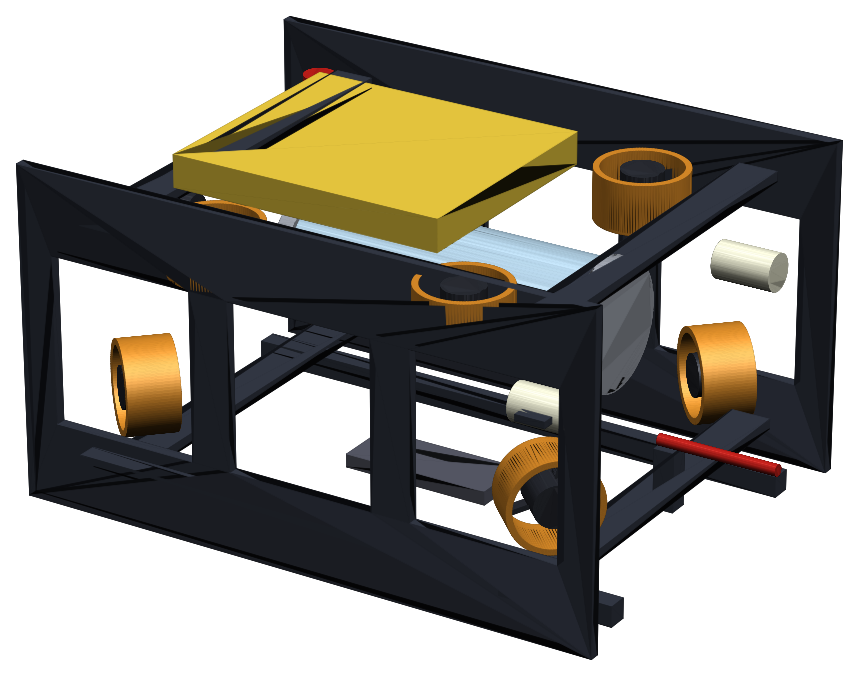
\includegraphics[width=0.62\linewidth]{../cad/isonavi_rov_hero.png}}{}

\vspace{3mm}
\begin{minipage}{0.94\linewidth}
\centering\footnotesize
\renewcommand{\arraystretch}{1.05}
\begin{tabular}{@{}lc@{\hspace{7mm}}lc@{}}
\toprule
Mass, envelope & \SI{\mmass}{\kilo\gram}, \mlenoverall{} x \mbeam{} x \mheight{} cm &
Contacts per run, murky: pilot, camera & \mrefmanualmurkycontacts{}, \mrefautomurkycontacts{} \\
Surge force, one unit lost & \SI{\msurgelost}{\newton} &
Contacts per run, turbid: assist, camera & \mrefassistmidcontacts{}, \mrefautomidcontacts{} \\
Governed input, peak current & \SI{\mcapw}{\watt}, \SI{\mpeakamps}{\ampere} &
Target colour, \SI{1}{\metre}, murky water & \midmurkyone{}\,\% \\
Link loss to zero thrust & \SI{\mholdtime}{\second} &
Cost, vehicle with tether and surface & \INR{\mcostbuild} \\
\bottomrule
\end{tabular}
\end{minipage}

\vfill
{\small Every number in this report is generated from the result files\\
by a script in the repository that accompanies it\\[1mm]
\texttt{github.com/AUV-VITP/isonavi-rov}}
\end{titlepage}

\tableofcontents
\newpage

% ======================================================================
\section{Requirements}

The vehicle is designed against the following, which together describe a
piloted pool task: pass a submerged gate without touching it, identify a
target by colour in an unlit pool and touch it, and fly a walled maze while
touching as little as possible.

\begin{table}[htbp]\centering\small
\begin{tabular}{@{}lll@{}}
\toprule
Requirement & Value & How it is met \\
\midrule
Mass in air & below \SI{35}{\kilo\gram}, target below \SI{20}{\kilo\gram} & \SI{\mmass}{\kilo\gram}, Section~\ref{sec:budget} \\
Envelope & target below 75 x 65 x 60 cm & \mlenoverall{} x \mbeam{} x \mheight{} cm over the probe \\
Power & 230 V 50 Hz mains, fused & 48 V supply, \SI{\mfuse}{\ampere} fuse, Section~\ref{sec:power} \\
Emergency stop & external kill switch & four layer chain, Section~\ref{sec:safety} \\
Tether & about \SI{50}{\metre} & power pair and Cat5e, neutrally buoyant \\
Pool & 20 x 10 m, 0.6 to 1.8 m deep & arena model, Section~\ref{sec:arena} \\
Gate & \SI{1}{\metre} clear opening & beam \SI{\mbeam}{\centi\metre} \\
Maze walls & up to \SI{1.5}{\metre} high, covered passage & arena model \\
Leaks and pollution & none & no battery aboard, sealed hull, leak probes \\
Compressed gas, lasers & none carried & not applicable \\
\bottomrule
\end{tabular}
\caption{Design requirements and where each is closed.}\label{tab:req}
\end{table}

\section{What carries over from isonavi, and what changes}

isonavi-1 is a \SI{28}{\kilo\gram} faired survey vehicle built to hold
station in a \SI{2.4}{\metre\per\second} flood current with acoustic
perception. A pool asks for the opposite: no current, depth under two metres,
targets identified by colour, and a narrow course flown by a person.

\begin{table}[htbp]\centering\small
\begin{tabular}{@{}p{0.27\linewidth}p{0.27\linewidth}p{0.38\linewidth}@{}}
\toprule
isonavi-1 & isonavi-rov & Reason \\
\midrule
Autonomous survey & Piloted, with assist and vision modes & A person flies it; the assist and vision loops are what reduce contacts \\
Faired 1074 mm hull with fins & Open frame, \mlenframe{} cm & No current; a holonomic box clears a \SI{1}{\metre} corridor \\
\SI{50}{\metre} rating, ring frames & One acrylic housing & Under two metres of water \\
Forward-looking sonar and DVL & Camera, two lamps, IMU, depth & Targets are told apart by colour, in the dark \\
\SI{1.5}{\kilo\watt\hour} battery aboard & 48 V down the tether & No battery and no battery leak aboard \\
Mission state machine & Pilot assist, governor, supervisor, ROS 2 & It must stop safely on a kill, a leak or a lost link \\
\bottomrule
\end{tabular}
\caption{The engines are kept; the vehicle and its perception are replaced.}
\end{table}

Unchanged and reused directly: the vectorised ray caster, which now forms
camera images instead of sonar images; the Fossen dynamics and the eight
thruster allocation; the cascade of solved budget, CAD check and generated
bill of materials; and the flight computer, ESP32 actuator interface and
framed protocol, extended by two message types.

% ======================================================================
\section{Vehicle}\label{sec:budget}

\keyfig{../cad/isonavi_rov_views.png}{General arrangement, from the CAD model
built out of the solved budget. Four horizontal thrusters canted at 45 degrees
give surge, sway and yaw; four vertical thrusters give heave, roll and pitch.
The vehicle can move sideways without turning, which is how it crosses the
slalom without widening its swept path.}{fig:views}

\subsection{Mass, buoyancy and trim are solved}

Every component is listed with a mass, a displaced volume and a station
(\texttt{cad/rov.py}). Three things are then solved rather than chosen: the
foam volume, so the vehicle floats \SI{\mnetbuoy}{\newton} positive and rises
if power is lost; the lead ballast, so the centre of gravity sits
\SI{\mbg}{\milli\metre} below the centre of buoyancy and the vehicle rights
itself; and the foam station, so it floats level (trim offset
\SI{\mtrim}{\milli\metre}). The result is \SI{\mmass}{\kilo\gram} and
\SI{\mdisplaced}{\litre} with \SI{\mfoam}{\litre} of foam and
\SI{\mballast}{\kilo\gram} of lead.

\subsection{The CAD checks the budget}

\texttt{cad/rov\_cad.py} builds the \mcadparts{}-part assembly from the solved
budget and checks it three ways. The displaced volume of each group as built
agrees with the budget: buoyancy \SI{\mcadbuoybuilt}{\litre} and hull
\SI{\mcadhullbuilt}{\litre} exactly, the rest to within items not modelled as
solids (fasteners, cables, the depth sensor). The assembly fits a
\mcadenvl{} x \mcadenvb{} x \mcadenvh{} cm box. And every part is tested
against every other for overlap: \mcadclash{} pairs overlap, the closest
thruster duct clears a side plate by \SI{\mcadplate}{\milli\metre}, and the
foam blocks \SI{\mcadoutflow}{\milli\litre} of the worst vertical thruster's
outflow.

The check earned its place. The first build found the vertical ducts
touching the side plates, which moved their station inboard by
\SI{15}{\milli\metre}; displaced volumes for the ducts, skids and end caps
that the budget had underestimated; a probe that protrudes
\SI{6}{\centi\metre} past the frame and therefore had to be in the contact
model; lamps that overlapped the front horizontal ducts; and a kill switch
inside the foam. Each was fixed in the budget, not only in the drawing, and
the simulation re-run.

\subsection{Hydrodynamics and thrust}

Damping and added mass are scaled from the tank-identified coefficients of
the open frame vehicle isonavi used as its reference, by projected area and
displaced volume. With \mthrustmax{}~N thrusters the vehicle makes
\SI{\msurgefull}{\newton} in surge and sway and \SI{\mheavefull}{\newton} in
heave, for \SI{\mspeedfull}{\metre\per\second} ahead.

The course is flown at \SI{\mopsspeed}{\metre\per\second}. There, the tether
is a third of the load: \mtrail{} m of trailing tether adds
\SI{\mtetherdrag}{\newton} to the frame's \SI{\mframedrag}{\newton}. With any
one thruster lost, a linear program over the surviving seven still makes
\SI{\msurgelost}{\newton} with zero net moment, a margin of \mopsmargin{} over
that load. That margin is what set the thrust target at \mthrustmax{}~N.

\subsection{Thrusters, made in house}

Each thruster is a hobby outrunner run flooded, with a potted stator, in a
printed Kort duct with a \SI{76}{\milli\metre} three blade propeller. The
motor is matched to the propeller rather than picked by habit
(\texttt{cad/thruster.py}): at the bench point the propeller turns at about
\mkvrpm{}~rpm, far below where a high KV winding wants to run, so the motor
works at low speed and high torque. A 1000~KV winding would carry
\SI{\mkvthousandphase}{\ampere} of phase current, past 80\,\% of a
\SI{30}{\ampere} controller. The \mkvchosen{}~KV winding carries
\SI{\mkvphase}{\ampere} and draws \SI{\mkvinput}{\watt}, and its motor and
propeller efficiencies together reproduce the drive efficiency the power path
was sized on.

% ======================================================================
\section{Power and tether}\label{sec:power}

A mains supply at the poolside makes \SI{48}{\volt}, which runs down two
paralleled \SI{2.5}{\milli\metre\squared} cores per leg (loop resistance
\SI{\mloopohm}{\ohm}) to two converters aboard that feed the thruster rail.
There is no battery on the vehicle.

All eight thrusters at full draw \SI{\muncapped}{\watt}, which would need a
\SI{40}{\ampere} fuse and a supply to match. That is not a design point, so a
governor in the allocator caps input at \SI{\mcapw}{\watt}. Propeller power
from momentum theory is homogeneous of degree $3/2$ in thrust, so scaling
every thruster by $k$ scales the total by $k^{3/2}$ and the $k$ that meets the
cap is exact in one step. At the cap all eight together still make
\SI{\mcapthrust}{\newton} each, the current is \SI{\mpeakamps}{\ampere}, the
converters see \SI{\mvinpeak}{\volt} against a \SI{36}{\volt} floor, and the
tether dissipates \SI{\mtetherloss}{\watt}. The surface supply is
\SI{\msupplyw}{\watt} and the main fuse \SI{\mfuse}{\ampere}, at 1.25 times
the governed peak current. Fifty metres is inside the \SI{100}{\metre} reach
of plain Ethernet, so the data pair is Cat5e with no modem.

% ======================================================================
\section{Safety chain}\label{sec:safety}

Four layers, each able to stop the thrusters on its own:
\begin{enumerate}
\item a fused mains supply with an emergency stop on its output;
\item an external magnet kill switch on the vehicle that opens the thruster rail;
\item the supervisor on the flight computer, which zeroes thrust on a kill, a
leak, or \SI{\mholdtimeout}{\second} without a pilot packet, and latches the
kill and leak states;
\item the ESP32, whose firmware drops every channel to neutral if the flight
computer goes quiet.
\end{enumerate}
The vehicle floats positive, so zero thrust is the safe state: from the
deepest point of the pool it rises unpowered. On the hardware-in-the-loop
bench (Section~\ref{sec:hil}) a \SI{10}{\second} loss of pilot packets put
the board in HOLD \SI{\mholdtime}{\second} after the last packet, one control
tick after the timeout, with zero thrust throughout and a rise of
\SI{\mholdrise}{\metre}; packets returning re-armed it. A kill latched on the
tick it arrived and held zero thrust for all \mkillticks{} ticks that
followed, through continuing pilot traffic.

% ======================================================================
\section{Arena and camera}\label{sec:arena}

\subsection{Arena}

The pool is \SI{20}{\metre} by \SI{10}{\metre}, its floor sloping from
\SI{0.6}{\metre} to \SI{1.8}{\metre}. The course is a gate of two posts and a
crossbar with a \SI{1}{\metre} opening; four balloons of different colours on
a line, one of which is the target; and a three section maze, a straight
corridor, a slalom between posts, and a covered passage, with walls up to
\SI{1.5}{\metre} high. Placement is parametric, and the results are reported
both for a reference layout and for forty layouts drawn at random. Each
element carries a signed distance function, and the hull and probe are
sampled as points, so a contact is any sample on or inside an element.

\subsection{Camera image formation}

In an unlit pool the only light is what the vehicle carries. Per pixel and
per colour channel, with $c$ the attenuation coefficient, $\beta$ the volume
backscatter coefficient, $\rho$ the surface albedo, $t$ the range along the
ray and $r_l$ the lamp to point range,
\begin{align*}
L &= \frac{\rho}{\pi} \sum_{\text{lamps}} I_0\, b(\theta) \cos i\, \frac{e^{-c r_l}}{r_l^2}\, e^{-c t}, &
B &= \int_0^t \beta \sum_{\text{lamps}} I_0\, b(\theta_s) \frac{e^{-c r_l(s)}}{r_l(s)^2}\, e^{-c s}\, ds .
\end{align*}
Red is absorbed several times faster than blue, so colour fails before
detection does, and the backscatter integral is evaluated along every ray, so
lamp placement shows in the image the way it does in a real one. Water clarity
is set by the scattering coefficient $b$: $0.05$ per metre for a clear pool,
$0.4$ for a turbid one and $1.0$ for murky water.

\keyfig{../simulation/results/figures/r3_camera_views.png}{The onboard camera
at the same pose in three water clarities, rendered by the camera model. In
murky water the balloons are still there; their colour is not.}{fig:cam}

% ======================================================================
\section{Vision}

\subsection{Target colour, without training data}

A fixed colour threshold works at one range in one water and nowhere else, so
the target finder undoes the water instead. It removes the backscatter veil,
segments what remains into round blobs, takes range from apparent size
against the known target radius, multiplies each channel by $e^{2cr}$ to undo
the two way attenuation at that range, and matches the corrected chromaticity
to the nearest reference. A blob whose size implies a range the lamps cannot
light is speckle and is rejected; left in, the correction at that range turns
it any colour.

With the lamps as built, \SI{0.18}{\metre} either side of the lens, the target
colour is identified at \SI{1}{\metre} in \midclearone{}, \midmidone{} and
\midmurkyone{}\,\% of frames in clear, turbid and murky water, and at
\SI{1.5}{\metre} in \midclearonehalf{}, \midmidonehalf{} and
\midmurkyonehalf{}\,\%. Lamp placement matters: at \SI{1.5}{\metre} in turbid
water, lamps \SI{0.10}{\metre} off the lens identify \mlampnarrowmid{}\,\% and
lamps as built \mlampbuiltmid{}\,\%. The operating rule that follows is to
close to about a metre before committing to a colour.

\keyfig{../simulation/results/figures/r2_target_identification.png}{Target
colour identified correctly against range, by water clarity and lamp
placement, from rendered frames at jittered poses.}{fig:id}

\subsection{Where the vehicle is on the course, from the image}

The camera mode measures the vehicle's position across the course from each
frame at \SI{5}{\hertz}, in \texttt{vision.}\allowbreak\texttt{CourseEstimator}:
\begin{itemize}
\item \textbf{gate and obstacles}: posts are found as narrow bright columns.
With the distance to the post known, each bearing, rotated by the IMU heading,
gives the lateral offset on its own, and an object elsewhere in the frame is
rejected by its bearing;
\item \textbf{target}: bearing and range from size of the detection of the
target colour;
\item \textbf{corridor}: a lamp-lit wall dims as the square of its distance,
so the log ratio of left to right wall brightness is
$s = 2 \ln\frac{w/2 + y}{w/2 - y}$ for an offset $y$ in a corridor of width
$w$. Inverted, $y = \frac{w}{2}\tanh(g s/4)$ plus a heading term; the gain
and heading term are fitted per water clarity on rendered frames from random
layouts and tested on held-out frames.
\end{itemize}

\begin{table}[htbp]\centering\small
\begin{tabular}{@{}lccc@{}}
\toprule
RMS lateral error, mm & $b = 0.05$ & $b = 0.4$ & $b = 1.0$ \\
\midrule
Corridor, straight section & \mwallclearstraight & \mwallmidstraight & \mwallmurkystraight \\
Corridor, covered passage & \mwallclearpassage & \mwallmidpassage & \mwallmurkypassage \\
Corridor walls, slalom section & \mwallclearobstacles & \mwallmidobstacles & \mwallmurkyobstacles \\
Posts, slalom section & \mpostsclear & \mpostsmid & \mpostsmurky \\
Gate posts at \SI{1}{\metre} & \mgateclearone & \mgatemidone & \mgatemurkyone \\
Target at \SI{1}{\metre} & \mtgtclearone & \mtgtmidone & \mtgtmurkyone \\
\bottomrule
\end{tabular}
\caption{Lateral position error of the course estimators on held-out rendered
frames. The slalom posts disturb the wall ratio, which is why that section
uses the posts.}\label{tab:est}
\end{table}

% ======================================================================
\section{Pilot in the loop}

The vehicle is flown by a person looking at the camera feed, so the question
is what a pilot with a reaction time, video latency and an imperfect read of
the picture achieves, and how much the vehicle's own loops change that. The
operator is a crossover model: stick commands are a gain on the perceived
error plus a lead term, delayed by \SI{0.25}{\second} of reaction and
\SI{0.15}{\second} of video latency, with motor noise on the stick. The
pilot's read of the course degrades with range and with the two way
attenuation of the vehicle's own light over it.

\begin{description}
\item[manual] sticks map to thrust; the pilot also flies depth and attitude,
which on a positively buoyant vehicle is constant work.
\item[assist] depth hold from the pressure sensor and heading and attitude
hold from the IMU; vertical speed is taken from the depth signal, not from
the simulator. The pilot steers in the horizontal plane only.
\item[camera] the assist loops plus the course estimators in the lateral loop,
rendered from the camera model every \SI{0.2}{\second}. Open water legs, with
nothing to see or hit, are held on heading, and progress along the course is
taken as known. On the vehicle the ROS~2 layer runs the corridor part of this
mode, which needs only the corridor width; gate and target guidance need the
course geometry, which the pilot supplies.
\end{description}
Runs are scored on what an observer records: contacts as events, the gate
passed clean or not, the right target touched with the probe or not, and time.

% ======================================================================
\section{Results}

\subsection{Reference layout}

\begin{table}[htbp]\centering\small
\begin{tabular}{@{}lccccc@{}}
\toprule
Mode, water & Finished & Gate clean & Right target & Contacts per run & Time, s \\
\midrule
manual, $b = 0.05$ & \mrefmanualcleardone/\mrefmanualclearn & \mrefmanualcleargate & \mrefmanualclearhit & \mrefmanualclearcontacts{} $\pm$ \mrefmanualclearcontactsd & \mrefmanualcleartime \\
manual, $b = 0.4$ & \mrefmanualmiddone/\mrefmanualmidn & \mrefmanualmidgate & \mrefmanualmidhit & \mrefmanualmidcontacts{} $\pm$ \mrefmanualmidcontactsd & \mrefmanualmidtime \\
manual, $b = 1.0$ & \mrefmanualmurkydone/\mrefmanualmurkyn & \mrefmanualmurkygate & \mrefmanualmurkyhit & \mrefmanualmurkycontacts{} $\pm$ \mrefmanualmurkycontactsd & \mrefmanualmurkytime \\
assist, $b = 0.05$ & \mrefassistcleardone/\mrefassistclearn & \mrefassistcleargate & \mrefassistclearhit & \mrefassistclearcontacts{} $\pm$ \mrefassistclearcontactsd & \mrefassistcleartime \\
assist, $b = 0.4$ & \mrefassistmiddone/\mrefassistmidn & \mrefassistmidgate & \mrefassistmidhit & \mrefassistmidcontacts{} $\pm$ \mrefassistmidcontactsd & \mrefassistmidtime \\
assist, $b = 1.0$ & \mrefassistmurkydone/\mrefassistmurkyn & \mrefassistmurkygate & \mrefassistmurkyhit & \mrefassistmurkycontacts{} $\pm$ \mrefassistmurkycontactsd & \mrefassistmurkytime \\
camera, $b = 0.05$ & \mrefautocleardone/\mrefautoclearn & \mrefautocleargate & \mrefautoclearhit & \mrefautoclearcontacts{} $\pm$ \mrefautoclearcontactsd & \mrefautocleartime \\
camera, $b = 0.4$ & \mrefautomiddone/\mrefautomidn & \mrefautomidgate & \mrefautomidhit & \mrefautomidcontacts{} $\pm$ \mrefautomidcontactsd & \mrefautomidtime \\
camera, $b = 1.0$ & \mrefautomurkydone/\mrefautomurkyn & \mrefautomurkygate & \mrefautomurkyhit & \mrefautomurkycontacts{} $\pm$ \mrefautomurkycontactsd & \mrefautomurkytime \\
\bottomrule
\end{tabular}
\caption{Course runs on the reference layout, 20 seeds per row.}\label{tab:ref}
\end{table}

Every run in every row finished and touched the right target. A pilot's
contacts are set by the water. In clear and turbid water a manual pilot
averages under one contact a run and the assist roughly halves that, because
the pilot no longer flies depth and attitude. At $b = 1.0$ the pilot's read
of the corridor fails with the two way attenuation of the vehicle's own
light, and contacts rise to \mrefmanualmurkycontacts{} manual and
\mrefassistmurkycontacts{} assisted, with a spread as large as the mean.

The camera mode behaves the other way. It makes \mrefautoclearcontacts{},
\mrefautomidcontacts{} and \mrefautomurkycontacts{} contacts a run at the
three clarities, with a small spread, because its error comes from the
estimators, which depend little on clarity, and not from a read that fails
with range. That is less than half the pilot's contacts in murky water and
several times more in clear and turbid water. The contacts are at the first
two slalom posts in every run traced. The gap beside a post is
\SI{\mslalomgap}{\centi\metre}, which leaves the \SI{\mbeam}{\centi\metre}
beam \SI{\mslalomside}{\milli\metre} a side when centred. There the wall
ratio, which assumes two plain walls, is disturbed by the posts
(\SI{\mwallmidobstacles}{\milli\metre} RMS at $b = 0.4$ against
\SI{\mwallmidstraight}{\milli\metre} in the straight section), and the post fit
is available in \mpostsmidavail\,\% of frames. In clear water the camera mode
also clips the gate in some runs (\mrefautocleargate{} of 20 clean): in
closed loop the gate estimate errs by \SI{\mrefautoclearvisgate}{\milli\metre}
RMS against \SI{\mgateclearone}{\milli\metre} at \SI{1}{\metre} on the held-out
frames of Table~\ref{tab:est}, because the vehicle arrives off the poses the
estimator was tested at, and the bright far wall competes with the posts.

The operating rule that follows is the one the ROS~2 pilot node implements:
the pilot flies, with the assist always on, and engages camera centring when
the water is too murky to read the course. Blending the camera's correction
with the pilot's stick, weighted by the error each has at that range and
clarity, is the next change to the camera mode; it is not done here.

\keyfig{../simulation/results/figures/r1_course_tracks.png}{Tracks of one seed
in each mode, in turbid and murky water; auto is the camera mode. Crosses mark
contacts.}{fig:tracks}


\subsection{Random layouts}

\begin{table}[htbp]\centering\small
\begin{tabular}{@{}lccccc@{}}
\toprule
Mode, water & Finished & Gate clean & Right target & Contacts per run & Time, s \\
\midrule
manual, $b = 0.4$ & \mlaymanualmiddone/\mlaymanualmidn & \mlaymanualmidgate & \mlaymanualmidhit & \mlaymanualmidcontacts{} $\pm$ \mlaymanualmidcontactsd & \mlaymanualmidtime \\
manual, $b = 1.0$ & \mlaymanualmurkydone/\mlaymanualmurkyn & \mlaymanualmurkygate & \mlaymanualmurkyhit & \mlaymanualmurkycontacts{} $\pm$ \mlaymanualmurkycontactsd & \mlaymanualmurkytime \\
assist, $b = 0.4$ & \mlayassistmiddone/\mlayassistmidn & \mlayassistmidgate & \mlayassistmidhit & \mlayassistmidcontacts{} $\pm$ \mlayassistmidcontactsd & \mlayassistmidtime \\
assist, $b = 1.0$ & \mlayassistmurkydone/\mlayassistmurkyn & \mlayassistmurkygate & \mlayassistmurkyhit & \mlayassistmurkycontacts{} $\pm$ \mlayassistmurkycontactsd & \mlayassistmurkytime \\
camera, $b = 0.4$ & \mlayautomiddone/\mlayautomidn & \mlayautomidgate & \mlayautomidhit & \mlayautomidcontacts{} $\pm$ \mlayautomidcontactsd & \mlayautomidtime \\
camera, $b = 1.0$ & \mlayautomurkydone/\mlayautomurkyn & \mlayautomurkygate & \mlayautomurkyhit & \mlayautomurkycontacts{} $\pm$ \mlayautomurkycontactsd & \mlayautomurkytime \\
\bottomrule
\end{tabular}
\caption{Forty random layouts per row: gate and target line placement, colour
order, which colour is the target, corridor width and slalom offsets all
vary.}\label{tab:lay}
\end{table}

The random layouts confirm the pattern. In turbid water the assist and the
manual pilot are close (\mlayassistmidcontacts{} and \mlaymanualmidcontacts{}
contacts a run) and the camera mode is behind (\mlayautomidcontacts{}, gate
clean in \mlayautomidgate{} of \mlayautomidn{}); in murky water the camera
mode makes \mlayautomurkycontacts{} against \mlaymanualmurkycontacts{} for
the manual pilot. The identification step is not where runs fail: the right
target was touched in every run, and a wrong target was touched first in
\mlaymanualmidwrong{} manual runs out of \mlaymanualmidn{} in turbid water.

% ======================================================================
\section{Hardware in the loop}\label{sec:hil}

The bench splits the loop the way the vehicle is wired. The host is the world
and the surface station: it holds the pool, the true dynamics and the sensor
models, runs the pilot, and sends the sensor sample and the pilot packet each
tick. The board is the vehicle: it runs the hold loops, the allocation, the
governor and the supervisor on what it receives and returns the wrench the
thrusters produce. It never sees the course or the truth. The protocol is
isonavi's framed, CRC-checked link with two message types added, the pilot
command and the supervisor report; a lost pilot packet is emulated by an
acknowledgement in its place, which keeps the bench deterministic.

Over the link, an assisted course finished in \SI{\mhiltime}{\second} against
\SI{\msimtime}{\second} in the pure simulation, with the same score
(\mhilcontacts{} contacts) and a largest position difference of
\SI{\mhildev}{\metre} over \mhilticks{} ticks, which is re-allocation round
off and nothing else. The safety results are in Section~\ref{sec:safety}.
The board and the ESP32 actuator interface are the units isonavi ran on
hardware; this bench ran over localhost, and the next step is the same run on
the boards.

% ======================================================================
\section{Software}

\begin{itemize}
\item \texttt{simulation/isonavi}: arena, camera, vision, pilot, safety, with
the isonavi dynamics, sensors and geometry they build on;
\item \texttt{ros/isonavi\_rov\_ros}: ROS~2 nodes for the pilot assist, the
safety chain, the actuator interface and vision, each a thin wrapper over the
module the simulation verified, including corridor centring from the wall
estimate in the auto mode. Built under Jazzy and run end to end: with
the gamepad live the actuator node emits the expected pulse widths, and when
it stops the supervisor reports HOLD and every channel goes to neutral;
\item \texttt{hil}: the bench in Section~\ref{sec:hil};
\item \texttt{cad}: budget, CAD and its checks, thruster match, bill of materials.
\end{itemize}

% ======================================================================
\section{Cost}

Prices are in rupees including GST, each line with the basis it rests on
(\texttt{cad/rov\_bom.py}).

\begin{table}[htbp]\centering\small
\begin{tabular}{@{}lr@{}}
\toprule
Group & Rupees \\
\midrule
Propulsion, eight thrusters & \mcostpropulsion \\
Hull & \mcosthull \\
Frame, foam and ballast & \mcostframe \\
Electronics & \mcostelectronics \\
\midrule
Vehicle & \mcostvehicle \\
Tether & \mcosttether \\
Surface station & \mcostsurface \\
\midrule
Vehicle, tether and surface & \mcostbuild \\
Test equipment and practice pool time & \mcosttest \\
Contingency & \mcostcont \\
\midrule
\textbf{Total} & \textbf{\mcosttotal} \\
\bottomrule
\end{tabular}
\caption{Cost by group. \minhouselines{} of \mbomlines{} lines are made in
house: the thrusters, end caps, frame, buoyancy, lamp housings, kill switch,
tether floats and the thrust rig.}\label{tab:cost}
\end{table}

% ======================================================================
\section{Verification and what remains}

Verified in simulation: the mass, buoyancy and trim budget against the CAD;
the thrust envelope with a unit lost; the power path at the governed peak;
target identification and the course estimators on rendered frames; the
course in three modes across water clarities and random layouts. Verified on
the bench: the vehicle-side software reproducing the simulation over the
link, and the safety chain under link loss and kill.

What needs water, in order:
\begin{enumerate}
\item a thrust curve for every thruster on the rig before it is fitted,
against the \mthrustmax{}~N target;
\item a vacuum test of the sealed hull, then a dunk test;
\item trim in a tank, against the solved foam and ballast;
\item camera frames in the pool to calibrate the attenuation coefficient and
the corridor gain, which the simulation takes from its model;
\item pilot hours on a mock course;
\item camera centring blended with the pilot's stick, so that the camera
mode is no worse than the assist in clear water.
\end{enumerate}
The hydrodynamic coefficients are scaled from a reference vehicle rather than
measured, and the operator model stands in for a real pilot; both are
replaced by measurement in the steps above.

\end{document}
